\documentclass[a4paper]{article}
\usepackage[utf8]{inputenc}

\usepackage{authblk}
\usepackage{setspace}
\renewcommand{\baselinestretch}{2.0} \usepackage[margin=1.25in]{geometry}
\usepackage{amsmath}
\usepackage{tabularx}
\usepackage{booktabs}
\usepackage{multirow}
\usepackage{makecell}
\usepackage{setspace}
\usepackage{siunitx}
\usepackage[backref]{hyperref}
\hypersetup{hidelinks} 
\usepackage{mathtools}
\usepackage{graphicx}
\usepackage{subfig} 
\graphicspath{{/home/ming/tools/latex2word/tests/en/temp_subtexfile_dir}} 
\title{An Example Test Document}

\author[1$\dag$]{Author A}
\author[1$\dag$]{Author B}
\author[1*]{Author C}
\author[1,2]{Author D}

\affil[1]{School of Example Studies, Example University}
\affil[2]{School of Advanced Example Studies, Example University}
\affil[*]{Address correspondence to: example.email@university.edu}
\affil[$\dag$]{These authors contributed equally to this work.}

\begin{document}

\maketitle

\begin{abstract}
This document provides a basic structure for an academic paper with test examples for tables, figures, formulas, and references. It includes examples of common LaTeX commands and document features.
\end{abstract}

\section{Introduction}

This document is a test example designed to help check various LaTeX formatting techniques, including tables, figures, and formulas. In the following sections, we will demonstrate these features.

\section{Tables}

There is a simple table in this section (Tab. \ref{tab:exampletable}).


\begin{table}[htbp]
    \centering
    \caption{
        An example table with parameters.
    }
    \label{tab:exampletable}
    \begin{tabular}{l}
    
\includegraphics[width=\linewidth]{tab_exampletable.png}
    \end{tabular}
\end{table}


Tab. \ref{table3} shows a more complex table.


\begin{table}[htbp]
    \centering
    \caption{Example Global Economic Indicators}
    \label{table3}
    \begin{tabular}{l}
    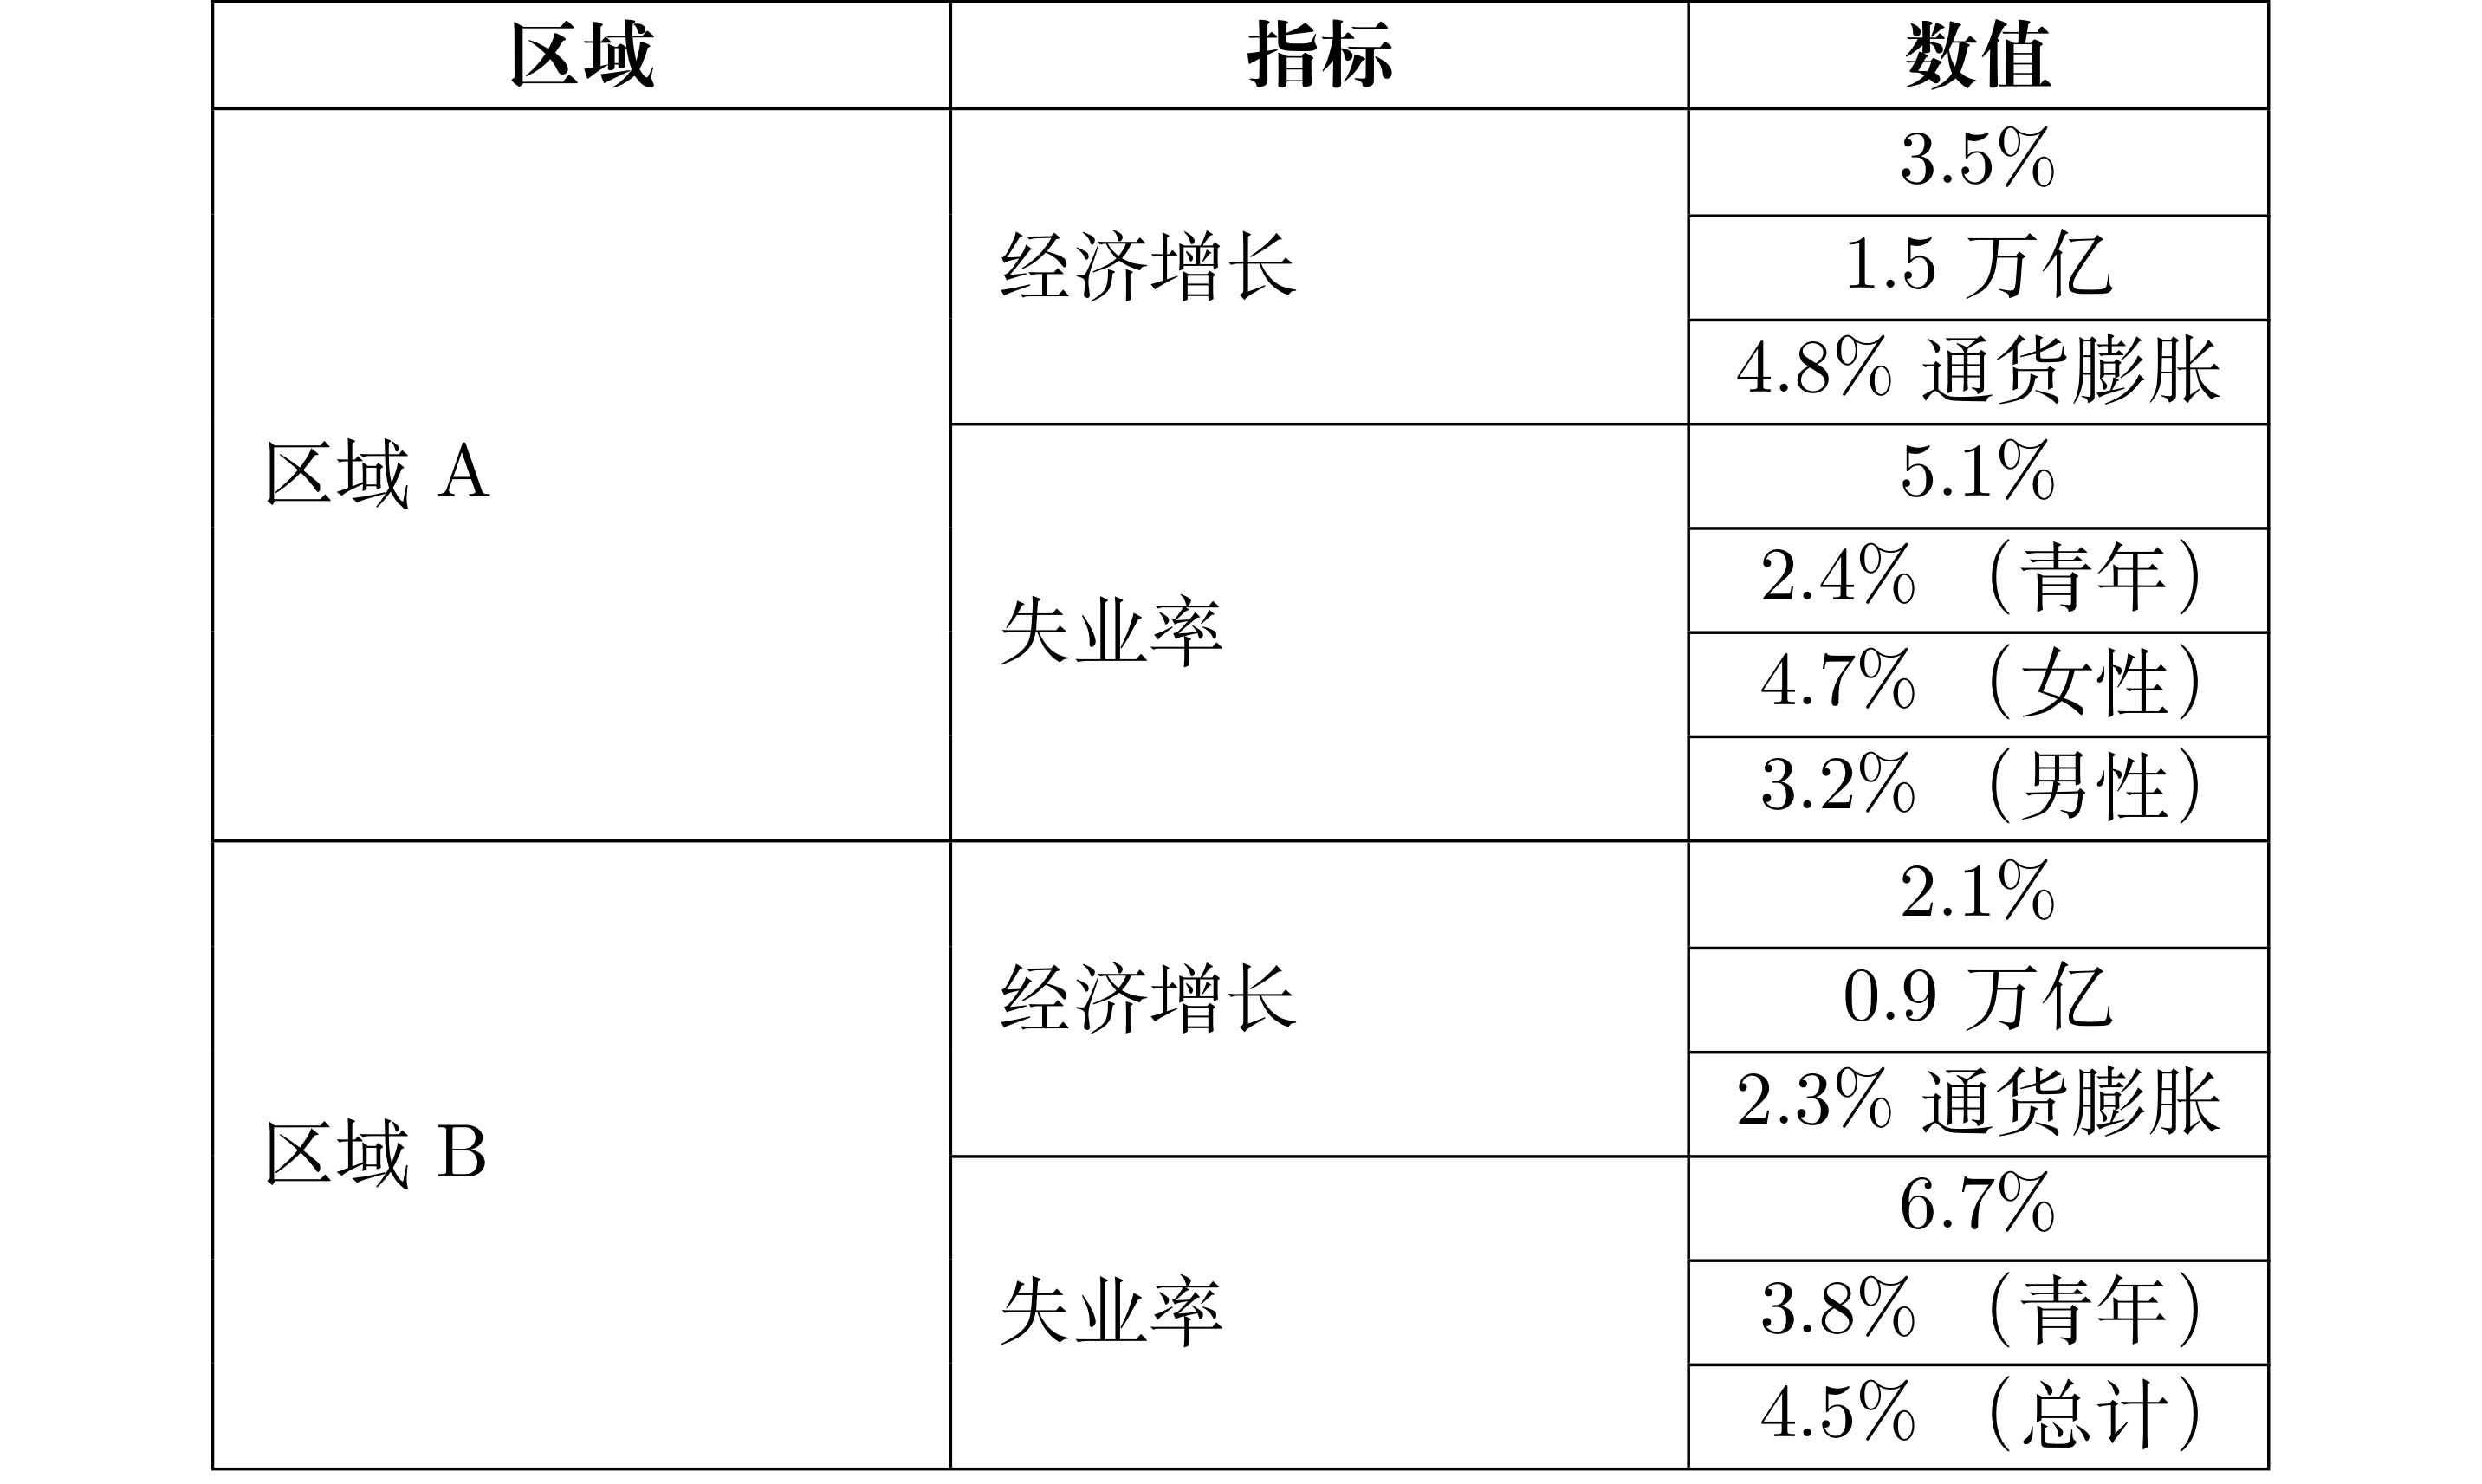
\includegraphics[width=\linewidth]{tab_table3.png}
    \end{tabular}
\end{table}



\section{Figures and their References}

\subsection{Example Figure}

Below is an example figure (Fig. \ref{multifig:multifig_examplefig}) showing a diagram that might represent a process or a conceptual flow.


\begin{figure}[htbp]
    \centering
    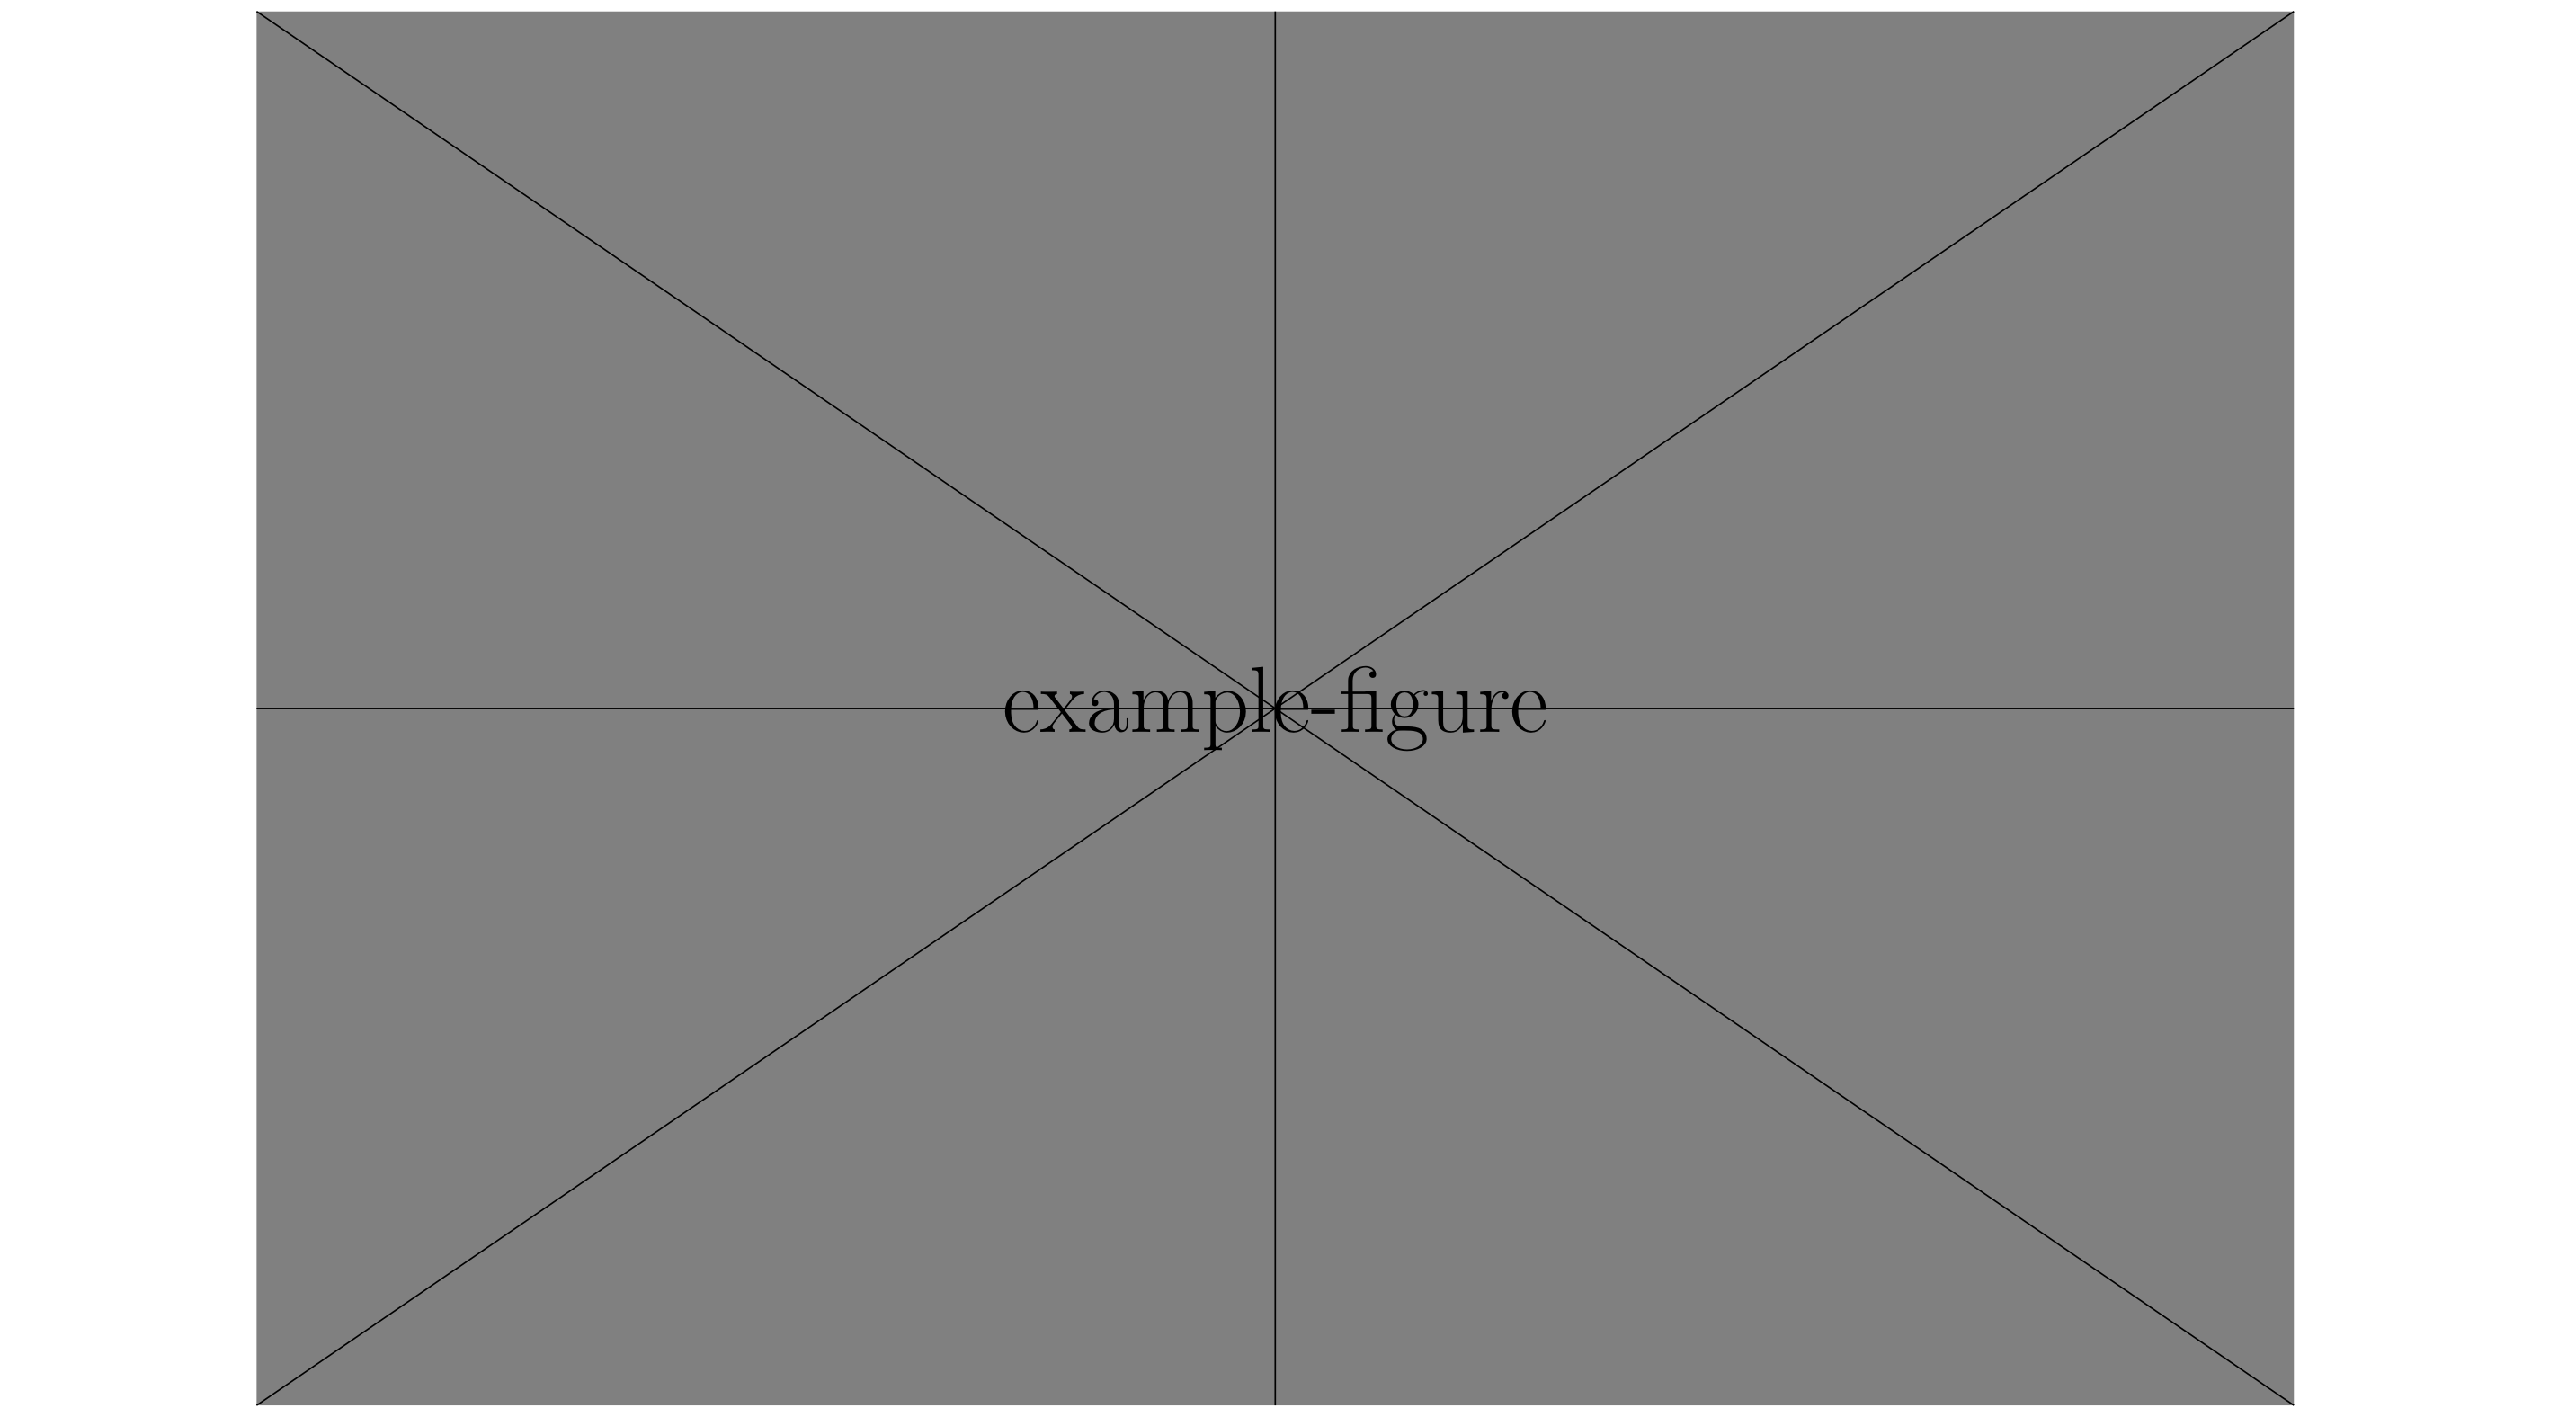
\includegraphics[width=\linewidth]{multifig_examplefig.png}
    \caption{
        An example figure showing a conceptual diagram.
    }
    \label{multifig:multifig_examplefig}
\end{figure}


\subsection{Subfigures}

Below is an example of subfigures (Fig. \ref{multifig:multifig_examplesubfigures}), which contains 4 subfigures (Fig. \ref{multifig:multifig_examplesubfigures}(a), Fig. \ref{multifig:multifig_examplesubfigures}(b), Fig. \ref{multifig:multifig_examplesubfigures}(c), and Fig. \ref{multifig:multifig_examplesubfigures}(d)).


\begin{figure}[htbp]
    \centering
    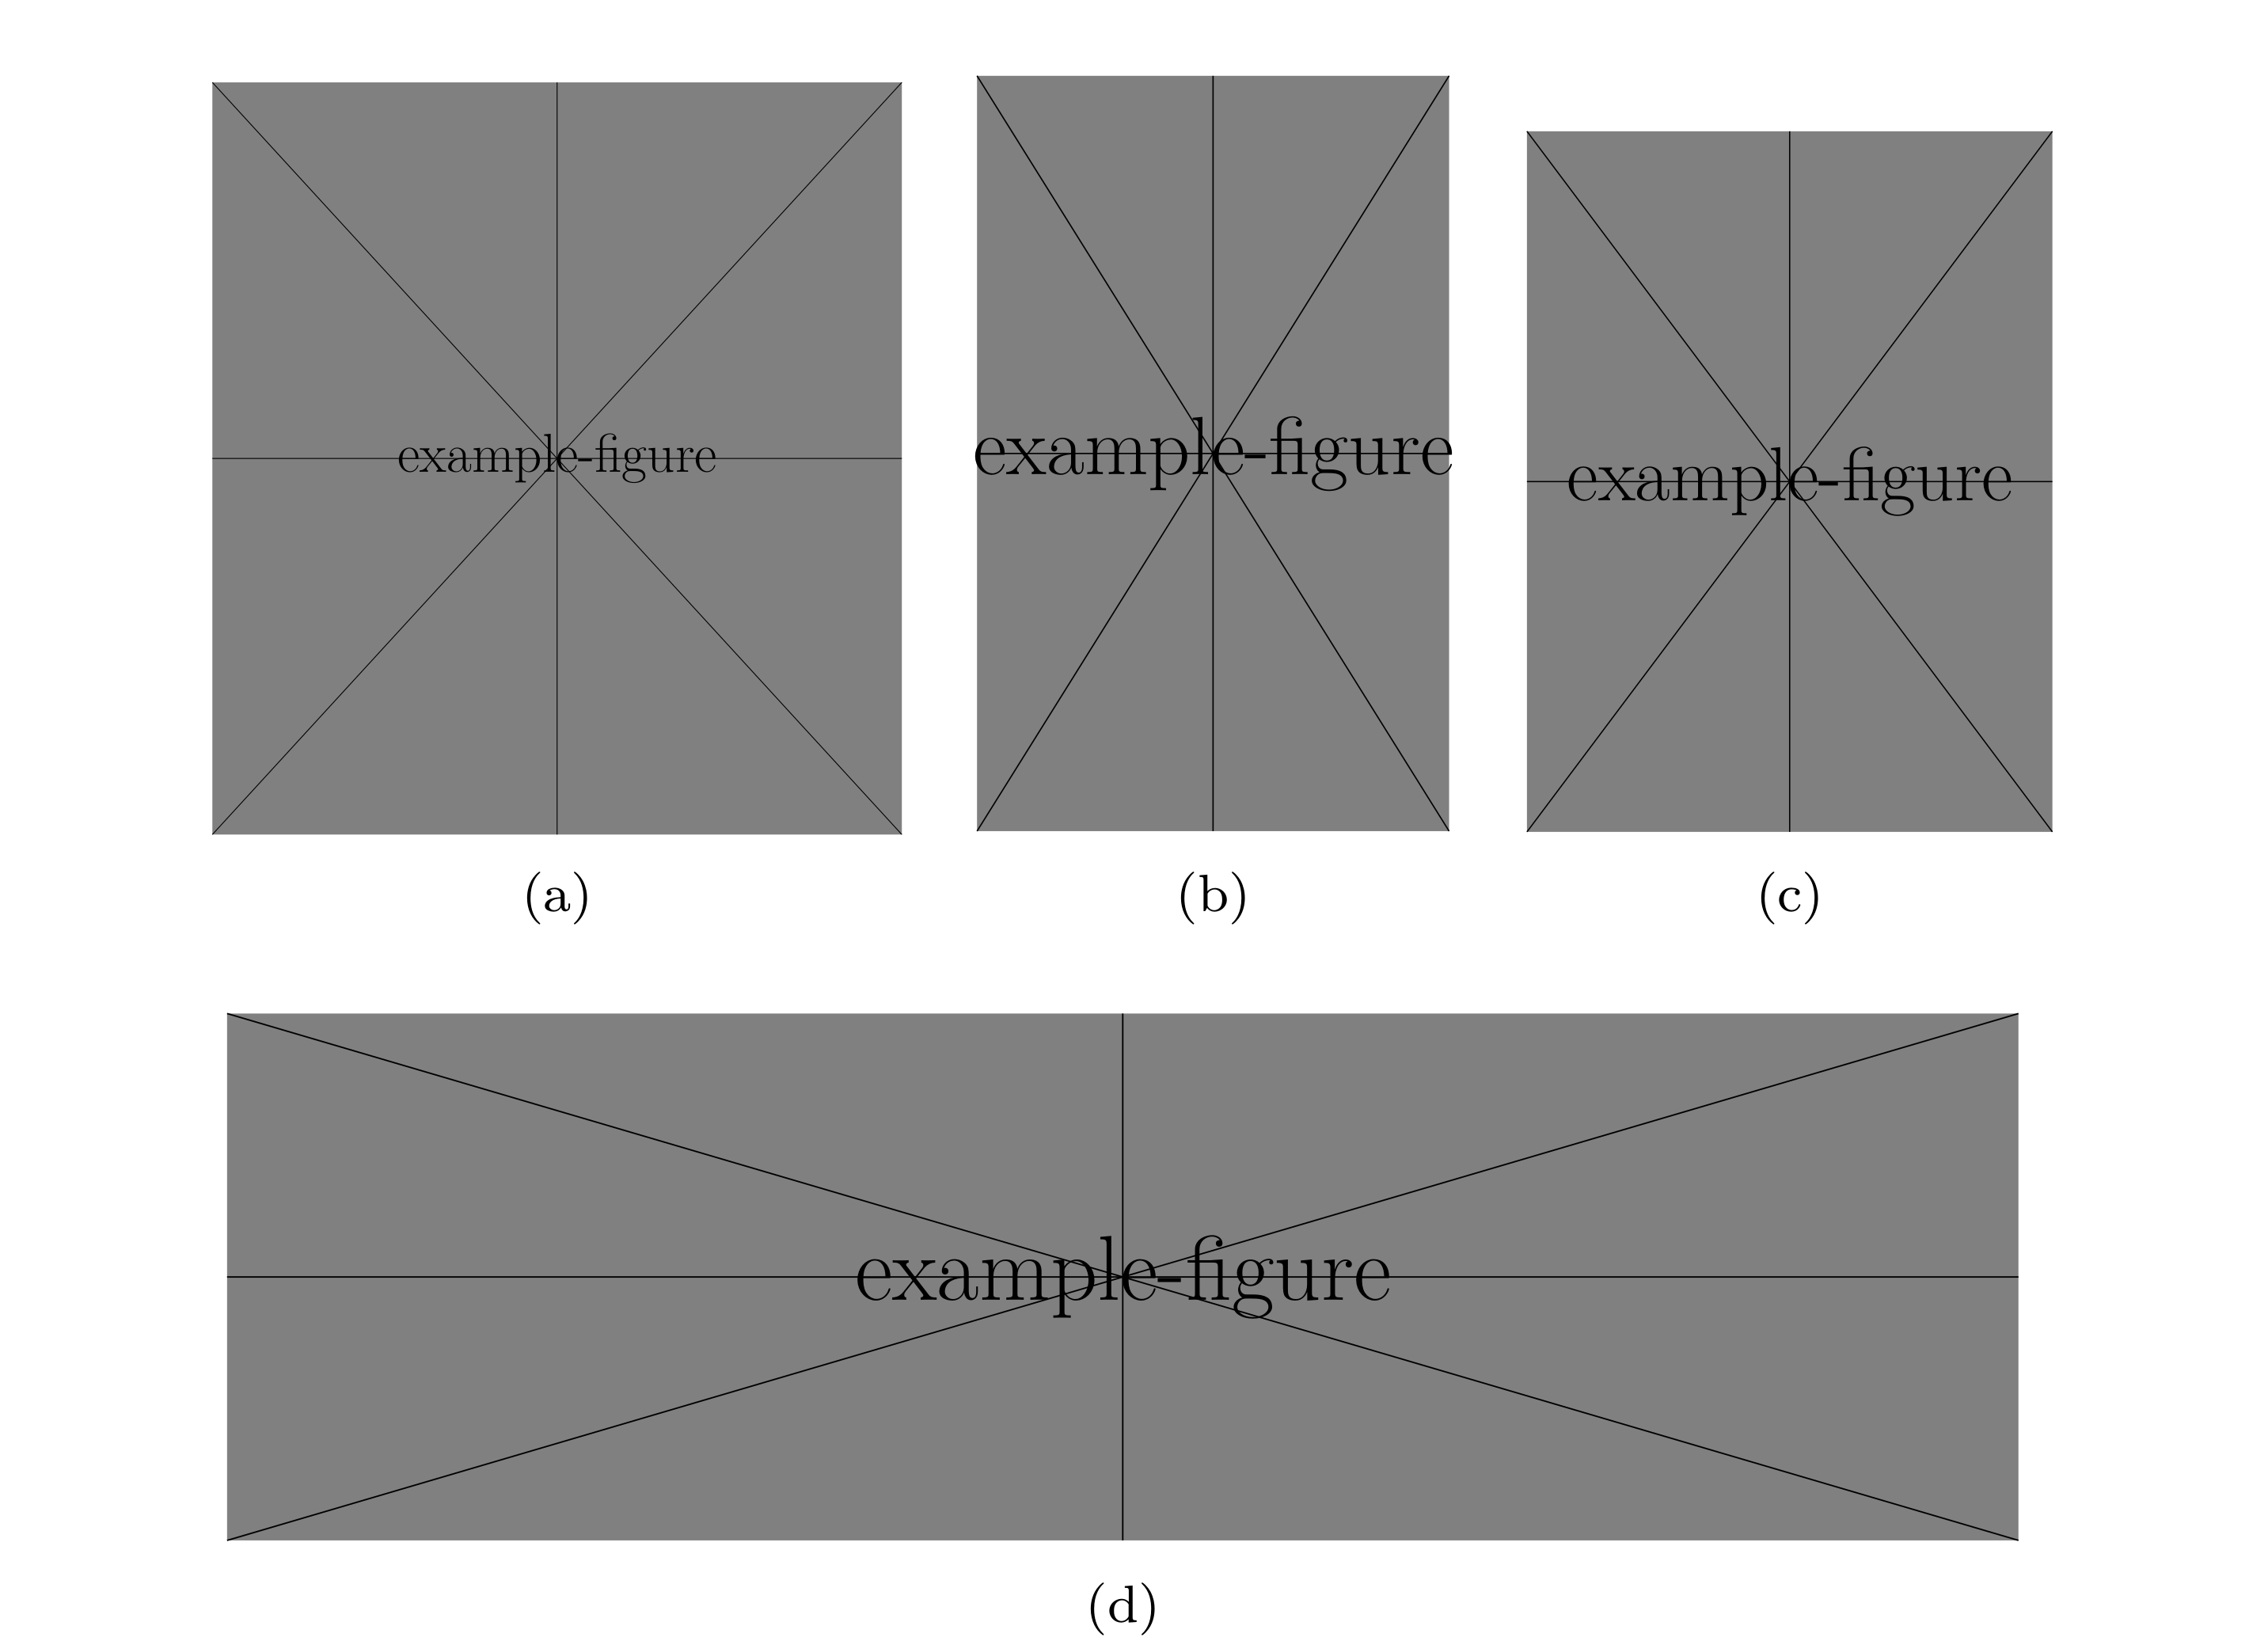
\includegraphics[width=\linewidth]{multifig_examplesubfigures.png}
    \caption{
        Example subfigures (a) Subfigure 1, (b) Subfigure 2, (c) Subfigure 3, and (d) Subfigure 4.
    }
    \label{multifig:multifig_examplesubfigures}
\end{figure}


\section{Formulas and Equations}

This section includes an example of how to format equations. The incidence matrix is given by Eq. \ref{eq:incidence}:

\begin{align}\label{eq:incidence}
    a_{kl}=
    \begin{cases}
        1,  & \text{edge $l$ leaves node $k$},\\
        -1, & \text{edge $l$ enters node $k$},\\
        0,  & \text{otherwise},
    \end{cases}
\end{align}
where $a_{kl}$ is the element of the incidence matrix, $k$ is the node index, and $l$ is the edge index.

\section{References}

This section includes an example of how to cite references\cite{article1}.

\bibliographystyle{ieeetr}
\bibliography{../ref}

\end{document}
